\documentclass[tikz]{standalone}
\usepackage{fourier}
\usepackage{tikz}

\begin{document}
	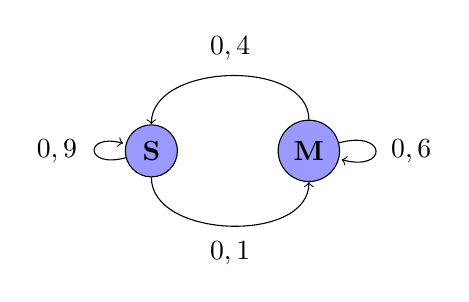
\begin{tikzpicture}
		\node[draw,circle,fill=blue!40!white](m) at (1,0) {\textbf{M}};
		\node[draw,circle,fill=blue!40!white](s) at (-1,0) {\textbf{S}};
		\node[draw=none] at (0,1.3) {$0,4$};
		\node[draw=none] at (2.3,0) {$0,6$};
		\node[draw=none] at (0,-1.3) {$0,1$};
		\node[draw=none] at (-2.2,0) {$0,9$};
		\draw[->] (m) edge [loop right] ();
		\draw[->] (s) edge [loop left] ();
		\draw[->] (m) to [out=90,in=90] (s);
		\draw[->] (s) to [out=-90,in=-90] (m);
	\end{tikzpicture}
\end{document}
